\documentclass{standalone}
\usepackage{tikz}
\usetikzlibrary{patterns, positioning}

\begin{document}
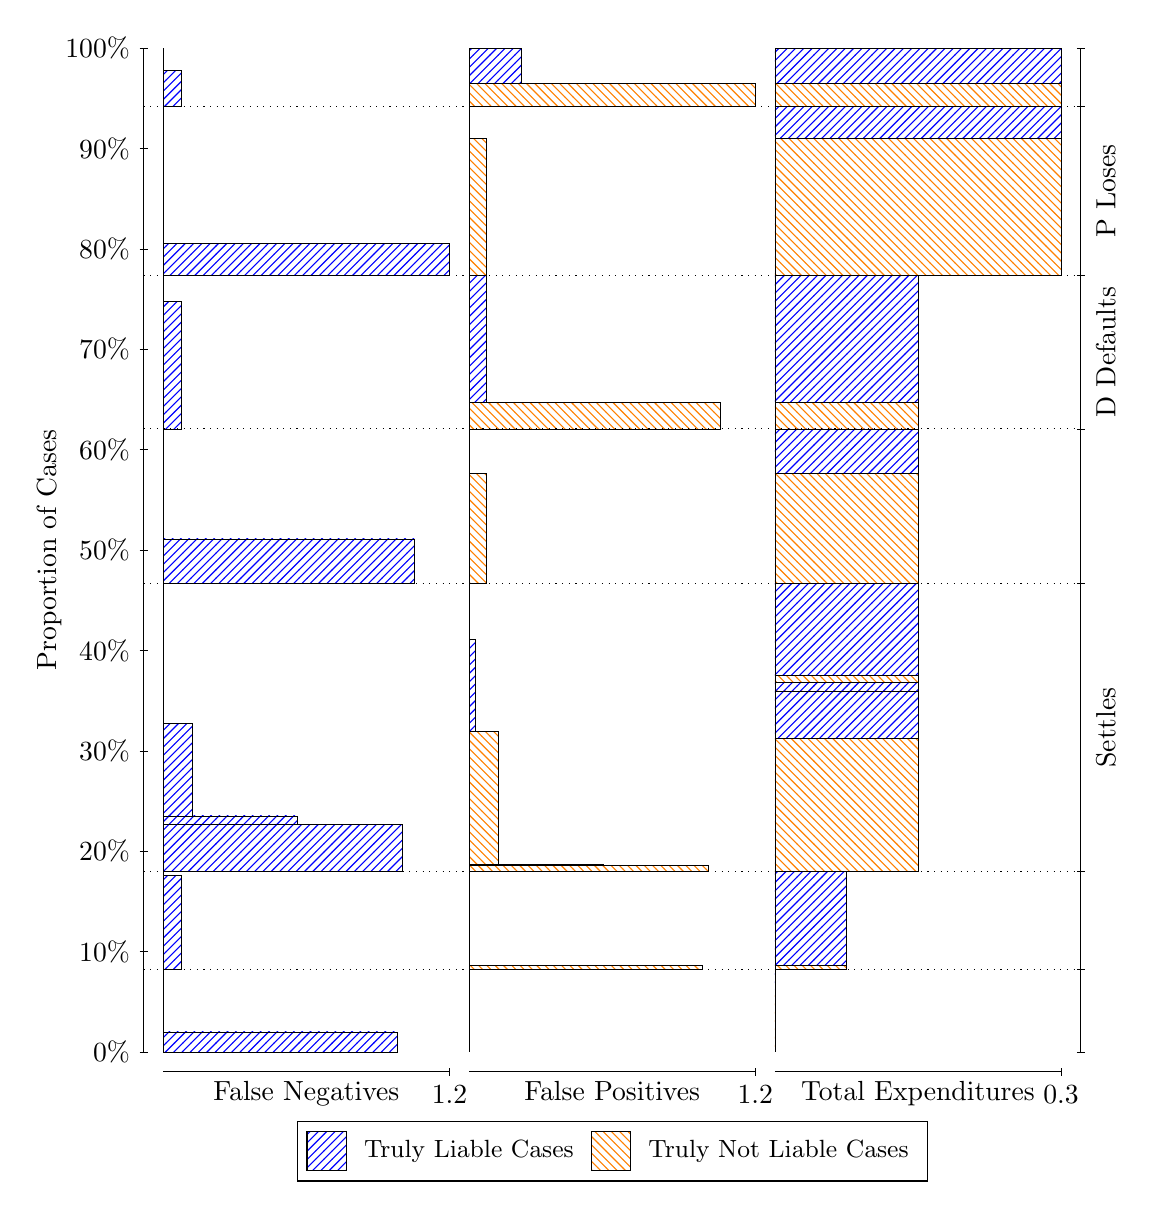
\begin{tikzpicture}
\draw[black, very thin] (1.5,1.75) -- (1.5,14.5);
\node[rotate=90, anchor=center] at (0.3, 8.125) {Proportion of Cases};
\draw[black, very thin] (1.45,1.75) -- (1.55,1.75);
\node[anchor=east] at (1.45, 1.75) {0\%};
\draw[black, very thin] (1.45,3.025) -- (1.55,3.025);
\node[anchor=east] at (1.45, 3.025) {10\%};
\draw[black, very thin] (1.45,4.3) -- (1.55,4.3);
\node[anchor=east] at (1.45, 4.3) {20\%};
\draw[black, very thin] (1.45,5.575) -- (1.55,5.575);
\node[anchor=east] at (1.45, 5.575) {30\%};
\draw[black, very thin] (1.45,6.85) -- (1.55,6.85);
\node[anchor=east] at (1.45, 6.85) {40\%};
\draw[black, very thin] (1.45,8.125) -- (1.55,8.125);
\node[anchor=east] at (1.45, 8.125) {50\%};
\draw[black, very thin] (1.45,9.4) -- (1.55,9.4);
\node[anchor=east] at (1.45, 9.4) {60\%};
\draw[black, very thin] (1.45,10.675) -- (1.55,10.675);
\node[anchor=east] at (1.45, 10.675) {70\%};
\draw[black, very thin] (1.45,11.95) -- (1.55,11.95);
\node[anchor=east] at (1.45, 11.95) {80\%};
\draw[black, very thin] (1.45,13.225) -- (1.55,13.225);
\node[anchor=east] at (1.45, 13.225) {90\%};
\draw[black, very thin] (1.45,14.5) -- (1.55,14.5);
\node[anchor=east] at (1.45, 14.5) {100\%};

\draw[black, very thin] (13.4,1.75) -- (13.4,14.5);
\draw[black, very thin] (13.35,1.75) -- (13.45,1.75);
\node[anchor=west] at (13.35, 1.75) {};
\draw[black, very thin] (13.35,2.7958) -- (13.45,2.7958);
\node[anchor=west] at (13.35, 2.7958) {};
\draw[black, very thin] (13.35,4.0404) -- (13.45,4.0404);
\node[anchor=west] at (13.35, 4.0404) {};
\draw[black, very thin] (13.35,7.6995) -- (13.45,7.6995);
\node[anchor=west] at (13.35, 7.6995) {};
\draw[black, very thin] (13.35,9.6643) -- (13.45,9.6643);
\node[anchor=west] at (13.35, 9.6643) {};
\draw[black, very thin] (13.35,11.613) -- (13.45,11.613);
\node[anchor=west] at (13.35, 11.613) {};
\draw[black, very thin] (13.35,13.762) -- (13.45,13.762);
\node[anchor=west] at (13.35, 13.762) {};
\draw[black, very thin] (13.35,14.5) -- (13.45,14.5);
\node[anchor=west] at (13.35, 14.5) {};

\draw[black, very thin, pattern color=blue, pattern=north east lines] (1.75,1.75) rectangle (4.716,2.0064);
\draw[black, very thin, pattern color=orange, pattern=north west lines] (1.75,2.0064) rectangle (1.75,2.7958);
\draw[black, very thin, pattern color=blue, pattern=north east lines] (1.75,2.7958) rectangle (1.9724,3.9899);
\draw[black, very thin, pattern color=orange, pattern=north west lines] (1.75,3.9899) rectangle (1.75,4.0404);
\draw[black, very thin, pattern color=blue, pattern=north east lines] (1.75,4.0404) rectangle (4.7901,4.6373);
\draw[black, very thin, pattern color=blue, pattern=north east lines] (1.75,4.6373) rectangle (3.4554,4.7497);
\draw[black, very thin, pattern color=blue, pattern=north east lines] (1.75,4.7497) rectangle (2.1207,5.9189);
\draw[black, very thin, pattern color=orange, pattern=north west lines] (1.75,5.9189) rectangle (1.75,7.6995);
\draw[black, very thin, pattern color=blue, pattern=north east lines] (1.75,7.6995) rectangle (4.9384,8.2667);
\draw[black, very thin, pattern color=orange, pattern=north west lines] (1.75,8.2667) rectangle (1.75,9.6643);
\draw[black, very thin, pattern color=blue, pattern=north east lines] (1.75,9.6643) rectangle (1.9724,11.281);
\draw[black, very thin, pattern color=orange, pattern=north west lines] (1.75,11.281) rectangle (1.75,11.613);
\draw[black, very thin, pattern color=blue, pattern=north east lines] (1.75,11.613) rectangle (5.3833,12.021);
\draw[black, very thin, pattern color=orange, pattern=north west lines] (1.75,12.021) rectangle (1.75,13.762);
\draw[black, very thin, pattern color=blue, pattern=north east lines] (1.75,13.762) rectangle (1.9724,14.216);
\draw[black, very thin, pattern color=orange, pattern=north west lines] (1.75,14.216) rectangle (1.75,14.5);
\draw[black, very thin, pattern color=orange, pattern=north west lines] (5.6333,1.75) rectangle (5.6333,2.5394);
\draw[black, very thin, pattern color=blue, pattern=north east lines] (5.6333,2.5394) rectangle (5.6333,2.7958);
\draw[black, very thin, pattern color=orange, pattern=north west lines] (5.6333,2.7958) rectangle (8.5993,2.8463);
\draw[black, very thin, pattern color=blue, pattern=north east lines] (5.6333,2.8463) rectangle (5.6333,4.0404);
\draw[black, very thin, pattern color=orange, pattern=north west lines] (5.6333,4.0404) rectangle (8.6735,4.1226);
\draw[black, very thin, pattern color=orange, pattern=north west lines] (5.6333,4.1226) rectangle (7.3388,4.1324);
\draw[black, very thin, pattern color=orange, pattern=north west lines] (5.6333,4.1324) rectangle (6.0041,5.821);
\draw[black, very thin, pattern color=blue, pattern=north east lines] (5.6333,5.821) rectangle (5.7075,6.9902);
\draw[black, very thin, pattern color=blue, pattern=north east lines] (5.6333,6.9902) rectangle (5.6333,7.6995);
\draw[black, very thin, pattern color=orange, pattern=north west lines] (5.6333,7.6995) rectangle (5.8558,9.0971);
\draw[black, very thin, pattern color=blue, pattern=north east lines] (5.6333,9.0971) rectangle (5.6333,9.6643);
\draw[black, very thin, pattern color=orange, pattern=north west lines] (5.6333,9.6643) rectangle (8.8218,9.9958);
\draw[black, very thin, pattern color=blue, pattern=north east lines] (5.6333,9.9958) rectangle (5.8558,11.613);
\draw[black, very thin, pattern color=orange, pattern=north west lines] (5.6333,11.613) rectangle (5.8558,13.354);
\draw[black, very thin, pattern color=blue, pattern=north east lines] (5.6333,13.354) rectangle (5.6333,13.762);
\draw[black, very thin, pattern color=orange, pattern=north west lines] (5.6333,13.762) rectangle (9.2667,14.046);
\draw[black, very thin, pattern color=blue, pattern=north east lines] (5.6333,14.046) rectangle (6.3007,14.5);
\draw[black, very thin, pattern color=orange, pattern=north west lines] (9.5167,1.75) rectangle (9.5167,2.5394);
\draw[black, very thin, pattern color=blue, pattern=north east lines] (9.5167,2.5394) rectangle (9.5167,2.7958);
\draw[black, very thin, pattern color=orange, pattern=north west lines] (9.5167,2.7958) rectangle (10.425,2.8463);
\draw[black, very thin, pattern color=blue, pattern=north east lines] (9.5167,2.8463) rectangle (10.425,4.0404);
\draw[black, very thin, pattern color=orange, pattern=north west lines] (9.5167,4.0404) rectangle (11.333,5.729);
\draw[black, very thin, pattern color=blue, pattern=north east lines] (9.5167,5.729) rectangle (11.333,6.3259);
\draw[black, very thin, pattern color=orange, pattern=north west lines] (9.5167,6.3259) rectangle (11.333,6.3357);
\draw[black, very thin, pattern color=blue, pattern=north east lines] (9.5167,6.3357) rectangle (11.333,6.4481);
\draw[black, very thin, pattern color=orange, pattern=north west lines] (9.5167,6.4481) rectangle (11.333,6.5303);
\draw[black, very thin, pattern color=blue, pattern=north east lines] (9.5167,6.5303) rectangle (11.333,7.6995);
\draw[black, very thin, pattern color=orange, pattern=north west lines] (9.5167,7.6995) rectangle (11.333,9.0971);
\draw[black, very thin, pattern color=blue, pattern=north east lines] (9.5167,9.0971) rectangle (11.333,9.6643);
\draw[black, very thin, pattern color=orange, pattern=north west lines] (9.5167,9.6643) rectangle (11.333,9.9958);
\draw[black, very thin, pattern color=blue, pattern=north east lines] (9.5167,9.9958) rectangle (11.333,11.613);
\draw[black, very thin, pattern color=orange, pattern=north west lines] (9.5167,11.613) rectangle (13.15,13.354);
\draw[black, very thin, pattern color=blue, pattern=north east lines] (9.5167,13.354) rectangle (13.15,13.762);
\draw[black, very thin, pattern color=orange, pattern=north west lines] (9.5167,13.762) rectangle (13.15,14.046);
\draw[black, very thin, pattern color=blue, pattern=north east lines] (9.5167,14.046) rectangle (13.15,14.5);
\draw[black, dotted] (1.5,2.7958) -- (13.4,2.7958);
\draw[black, dotted] (1.5,4.0404) -- (13.4,4.0404);
\draw[black, dotted] (1.5,7.6995) -- (13.4,7.6995);
\draw[black, dotted] (1.5,9.6643) -- (13.4,9.6643);
\draw[black, dotted] (1.5,11.613) -- (13.4,11.613);
\draw[black, dotted] (1.5,13.762) -- (13.4,13.762);
\draw[black, very thin] (1.75,1.5) -- (5.3833,1.5);
\node[anchor=north] at (3.5667, 1.5) {False Negatives};
\draw[black, very thin] (5.3833,1.45) -- (5.3833,1.55);
\node[anchor=north] at (5.3833, 1.45) {1.2};

\draw[black, very thin] (5.6333,1.5) -- (9.2667,1.5);
\node[anchor=north] at (7.45, 1.5) {False Positives};
\draw[black, very thin] (9.2667,1.45) -- (9.2667,1.55);
\node[anchor=north] at (9.2667, 1.45) {1.2};

\draw[black, very thin] (9.5167,1.5) -- (13.15,1.5);
\node[anchor=north] at (11.333, 1.5) {Total Expenditures};
\draw[black, very thin] (13.15,1.45) -- (13.15,1.55);
\node[anchor=north] at (13.15, 1.45) {0.3};



\node[black, centered, rotate=90] at (13.72, 5.87) {Settles};

\node[black, centered, rotate=90] at (13.72, 10.639) {D Defaults};
\node[black, centered, rotate=90] at (13.72, 12.687) {P Loses};


\draw (7.449999999999999,1.5) node[draw=none] (baseCoordinate) {};
\begin{scope}[align=center]
        \matrix[scale=0.5, draw=black, below=0.5cm of baseCoordinate, nodes={draw}, column sep=0.1cm]{
            \node[rectangle, draw, minimum width=0.5cm, minimum height=0.5cm, pattern=north east lines, pattern color=blue] {}; &
            \node[draw=none, font=\small] (B) {Truly Liable Cases}; &
            \node[rectangle, draw, minimum width=0.5cm, minimum height=0.5cm, pattern=north west lines, pattern color=orange] {}; &
            \node[draw=none, font=\small] (B) {Truly Not Liable Cases}; \\
            };
\end{scope}

\end{tikzpicture}
\end{document}